The diagram (Figure 1) below shows the basic architectural layer diagram of the Beverage Management app. The overall structure of our app can be described using the popular three-layer architecture which consists of presentation layer, application layer and data access layer. The presentation layer is the top-most layer of our system which allows user to interact with the system. Application layer acts as an interface between the presentation layer and data access layer. This layer supports all of the core functions of our application. The data access layer is the layer where all the data and information are stored or retrieved from the database. In other words, the presentation layer takes input from the user and pass it to the application layer. The application layer then process those commands and pass the information to the data access layer. The data access layer either store the information on the database or retrieve the requested information from the database and pass it back to the application layer, and eventually to the presentation layer where the result is displayed in a user understandable format. 

\begin{figure}[h!]
	\centering
 	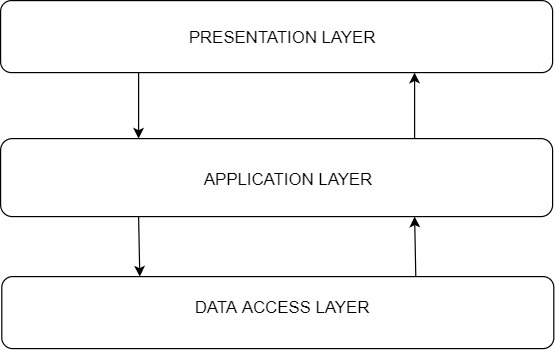
\includegraphics[width=0.60\textwidth]{images/ADS}
 \caption{A simple architectural layer diagram}
\end{figure}

\subsection{Layer X Description}
Each layer should be described separately in detail. Descriptions should include the features, functions, critical interfaces and interactions of the layer. The description should clearly define the services that the layer provides. Also include any conventions that your team will use in describing the structure: naming conventions for layers, subsystems, modules, and data flows; interface specifications; how layers and subsystems are defined; etc. 

\subsection{Layer Y Description}
Each layer should be described separately in detail. Descriptions should include the features, functions, critical interfaces and interactions of the layer. The description should clearly define the services that the layer provides. Also include any conventions that your team will use in describing the structure: naming conventions for layers, subsystems, modules, and data flows; interface specifications; how layers and subsystems are defined; etc. 

\subsection{Layer Z Description}
Each layer should be described separately in detail. Descriptions should include the features, functions, critical interfaces and interactions of the layer. The description should clearly define the services that the layer provides. Also include any conventions that your team will use in describing the structure: naming conventions for layers, subsystems, modules, and data flows; interface specifications; how layers and subsystems are defined; etc. 